
\documentclass[dvipdfmx]{standalone}
\usepackage[T1]{fontenc}
\usepackage{newtxtext, newtxmath}

\usepackage{tikz}
\usetikzlibrary{calc, intersections, through, backgrounds}

\begin{document}
  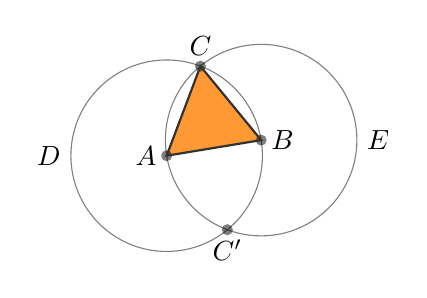
\begin{tikzpicture}[thick]
    \tikzset{
      help lines/.style={thin, draw=black!50},
    }
    \coordinate [label=left:$A$]  (A) at ($ (0,0) + .1*(rand,rand) $);
    \coordinate [label=right:$B$] (B) at ($ (1.25,0.25) + .1*(rand,rand) $);
    \node [name path=D, help lines, draw, label=left:$D$]  (D) at (A) [circle through=(B)] {};
    \node [name path=E, help lines, draw, label=right:$E$] (E) at (B) [circle through=(A)] {};
    \path [name intersections={of=D and E}]
      (intersection-1) coordinate (C) node [above] {$C$}
      (intersection-2) coordinate (C2) node [below] {$C'$};

    \foreach \point in {A,B,C,C2}
      \fill [black, opacity=.5] (\point) circle (2pt);
    \draw [black!80] (A) -- (C) -- (B) -- cycle;
    \begin{scope}[on background layer]
      \fill[orange!80] (A) -- (C) -- (B) -- cycle;
    \end{scope}
  \end{tikzpicture}
\end{document}
